% Created 2019-03-13 Wed 20:59
\documentclass{article}
\usepackage[utf8]{inputenc}
\usepackage[T1]{fontenc}
\usepackage{fixltx2e}
\usepackage{graphicx}
\usepackage{longtable}
\usepackage{float}
\usepackage{wrapfig}
\usepackage{rotating}
\usepackage[normalem]{ulem}
\usepackage{amsmath}
\usepackage{textcomp}
\usepackage{marvosym}
\usepackage{wasysym}
\usepackage{amssymb}
\usepackage{hyperref}
\usepackage{bm}
\usepackage{mystyle}
\DeclarePairedDelimiter{\diagfences}{(}{)}
\newcommand{\diag}{\operatorname{diag}\diagfences}
\tolerance=1000
\author{Dong Liu}

\usepackage{tikz}
\usetikzlibrary{calc,shapes,positioning}
\usetikzlibrary{arrows}
\newcommand{\midarrow}{\tikz \draw[-triangle 90] (0,0) -- +(.1,0);}

\title{alpha-EP for MIMO}
\hypersetup{
  pdfkeywords={},
  pdfsubject={},
  pdfcreator={Emacs 25.3.2 (Org mode 8.2.10)}}

\begin{document}
\maketitle
\tableofcontents


\section{Preview}
A fast preview of content of this manuscript:
\begin{itemize}
\item[\checkmark] Expectation Propagation (EP)
\item[\checkmark] PowerEP and alpha-EP
  \begin{itemize}
  \item[\checkmark] show improvement
  \end{itemize}
\item[\checkmark] Improvement/correction trick of EP
  \begin{itemize}
  \item[\checkmark] First order correction
  \item[$\times$] Do not suggest
  \end{itemize}
  
\item[\checkmark] Stochastic EP
  \begin{itemize}
  \item[-] simpler model, similar a bit worse performance than EP
  \end{itemize}
\item[\checkmark] Expectation Consistency
  
  \begin{itemize}
  \item[\checkmark] Single Loop
    \begin{itemize}
    \item[$?$] Improvement suggestion: full 2-order statistics, to Joao with low investigation priority
    \end{itemize}
    
  \item[$?$] Double Loop
    \begin{itemize}
    \item[-] Not really suggest for its complexity
    \end{itemize}
    
  \end{itemize}
  
  
\end{itemize}
\begin{itemize}
\item[$\times$] LU decomposition (Nima)
\item[\checkmark] Assembling/Boosting, mono-combination
  \begin{itemize}
  \item[$\times$] Assembling LU decomposition with permutation (Joao)
  \item[$\times$] Assembling multiple GTA approximations (Joao)
  
    
  \end{itemize}
\item[\checkmark] Assembling/Boosting, mix-combination (Nima)
  \begin{itemize}
  \item[\checkmark] GTA + EP
  \item[\checkmark] GTA-SIC + EP
  \end{itemize}

\end{itemize}

$\alpha$-BP
\section{Problem}\label{sec:problem}
The problem setting is the for observable signal $\bm{y}$, there is a true underlining signal $\bm{x}$ that results in the observation $\bm{y}$. Here $\bm{x}$ is assumed to lie in a discrete finite set, i.e. $\bm{x} \in {\Aa}^{N}$ and we denote its $i$-th element $x_i \in \Aa$. $\bm{y}\in \RR^N$. The further assumption between the relationship between $\bm{y}$ and $\bm{x}$ is linear with Gaussian noise $\bm{w}$, i.e. $\bm{w}\sim \Nn(\bm{0}, \sigma_{w}^2 \bm{I})$. The linear can be formulated as:
\begin{equation}\label{eq:linear-model}
  \bm{y} = \bm{H} \bm{x} + \bm{w}.
\end{equation}
The optimal way to estimate $\bm{x}$ is to look for the maximum a posterior (MAP) to
\begin{equation}
  p(\bm{x}|\bm{y}) \sim \Nn(\bm{y}: \bm{H}\bm{x}, \sigma_{w}^2\bm{I})\delta_{\bm{x}\in \Aa}.
\end{equation}
To avoid the complex computation, the original posterior is factorized into
\begin{equation}
  p(\bm{x}|\bm{y}) = \prod_i t_i(\bm{x}).
\end{equation}
Then, we try solve the problem with an approximated distribution 
\begin{equation}\label{eq:apx-dist-q}
  q(\bm{x}) = \prod_i \tilde{t}_i(\bm{x}).
\end{equation}

------------------------

\begin{itemize}
\item[] Initialize $q(x)$ to optimize.
\item[] Repeat till convergence:\\
  For $i$ component in $q$:
  \begin{align}
    q^{\backslash i}(x) &= q(x) / \tilde{t}_i(x)\\
    % q^{new}(x)  &= \argmin_{\tilde{t}_i(x)} D_{\alpha}(t_i(x)q^{\backslash i}(x)\| q(x)) \\
    \tilde{t}^{new}(x) &= q^{new}(x)/q^{\backslash i}(x)
  \end{align}
\end{itemize}    

\section{Expectation Propagation (EP)} \label{sec:EP}
For the EP algorithm, we basically follow \cite{cespedes2014mimo} to establish a baseline algorithm.
In this algorithm, the approximated distribution is assumed to be:
\begin{equation}\label{eq:q-ep}
  q(\bm{x}) \sim \Nn(\bm{y}: \bm{H}\bm{x}, \sigma_{w}^2\bm{I}) \prod_{i=1}^{N} \exp\left( \gamma_i x_i - \frac{1}{2}\Lambda_i x_i^2 \right),
\end{equation}
where $\gamma_i \in \RR$ and $\Lambda_i \in \RR^{+}$ are the parameters to be estimated in EP. It is clear that $q(\bm{x})$ in \eqref{eq:q-ep} belongs to exponential family, Gaussian distribution to be specific:
\begin{equation}
  q(\bm{x}) \sim \Nn\left(\bm{x}:\bm{\mu}, \bm{\Sigma} \right),
\end{equation}
where we have its distribution parameter as
\begin{align}
  \bm{\Sigma} &= \left( \sigma_{w}^2\bm{H}^{T}\bm{H} +  \diag{\bm{\Lambda}} \right)^{-1}, \\
  \bm{\mu} & = \bm{\Sigma}\left( \sigma_{w}^2\bm{H}^{T}\bm{y} +  \bm{\gamma} \right).
\end{align}
where $\diag{\Lambda}$ is a diagnal matrix with $\Lambda_i$ as diagnal elements, $\bm{\gamma}=[\gamma_1, \gamma_2, \cdots, \gamma_N]^{T}$.

The EP algorithm keeps updating the parameters of $q(\bm{x})$ until it meets the stop criteria, after which the most probable $\bm{x}$ is estimated by using updated $q(\bm{x})$. To be specific, the iterations of EP can be detailed as follows:
\begin{itemize}
\item Update the marginal distribution of the cavity distribution at iteration $t$:
  \begin{equation}
    q^{(l)\backslash i}(u_i) = \frac{q^{(l)(u_i)}}{\exp\left( \gamma_i^{(l)}u_i - \frac{1}{2}\Lambda_i^{(l)}u_i^2 \right)} ,
  \end{equation}
  which is a Gaussian distribution. Let us denote this distribution as $q^{(l)\backslash i}(u_i) = \Nn\left( u_i: t_i^{(l)}, h_i^{2(l)} \right)$, with
  \begin{align}
    h_i^{2 (l)} &= \frac{\sigma_i^{2 (l)}}{1-\sigma_i^{2 (l)} \Lambda_i^{(l)}}, \\
    t_i^{(l)} &= h_i^{2(l)}\left( \frac{\mu_i^{(l)}}{\sigma_i^{2(l)}} - {\gamma_i^{(l)}} \right).
  \end{align}
  

\item Corresponding marginal distribution of cavity distribution of $p(\bm{x})$:
  \begin{equation}
    \hat{p}^{(l)}(u_i) \sim q^{(l)\backslash i}(u_i)\delta_{u_i \in \Aa_i}.
  \end{equation}
\item Update the statistics parameter $\left( \bm{\gamma}, \bm{\Lambda} \right)$ of $q$, where the marginal distribution:
  \begin{equation}
    q^{(l+1)\backslash i}(u_i) \sim q^{(l)\backslash i}(u_i) \exp\left\{ \gamma_i^{(l+1)}u_i - \frac{1}{2}\Lambda_i^{(l+1)}u_i^2 \right\},
  \end{equation}
  where $q^{(t+1)\backslash i}(u_i)$ is parameterized by $\left(\bm{\gamma}, \bm{\Lambda}\right)$. This pair can be updated by:
  \begin{align}
    \Lambda_i^{(l+1)} = \frac{1}{\sigma_{p_i}^{2(l)}} - \frac{1}{h_i^{2(l)}} \\
    \gamma_i^{(l+1)} = \frac{\mu_{p_i}^{(t)}}{\sigma_{p_i}^{2(t)}} - \frac{t_i^{(t)}}{h_i^{2(t)}}.
  \end{align}
  
\end{itemize}

When stop criteria is meet, estimation is made by using $q(\bm{x}) \sim \Nn\left(\bm{x}:\bm{\mu}^{\ast}, \bm{\Sigma}^{\ast} \right)$, where
\begin{align}
  \bm{\Sigma}^{\ast} &= \left( \sigma_{w}^2\bm{H}^{T}\bm{H} +  \diag{\bm{\Lambda}^{\ast}} \right)^{-1}, \\
  \bm{\mu}^{\ast} & = \bm{\Sigma}^{\ast}\left( \sigma_{w}^2\bm{H}^{T}\bm{y} +  \bm{\gamma}^{\ast} \right)
\end{align}
are returned by the above EP iterations. The decision is made by:
\begin{equation}
  \hat{\mu}_{i} = \uargmin{\mu_i \in \Aa} \abs{\mu_i - \mu_i^{\ast}}
\end{equation}

\section{Power EP}\label{sec:power-ep}
In this section, we explain a variant of EP algorithm, known as power EP in literature \cite{minka2004power}.
Power EP has similar procedure of update as EP has. We would mainly discuss the difference here.

The power EP algorithm stems from a alpha-deiverge:
\begin{equation}
  D_{\alpha}(p\|q) = \frac{4}{1-\alpha^2} \left( 1 - \int_x p^{(1+\alpha)/2} q^{(1-\alpha)/2} \right)
\end{equation}

The meta algorithm of power EP can be summarize in high level steps as follows.
\begin{itemize}
\item Initialize $q(\bm{x}) \sim t_0(\bm{x})\prod_{i}\tilde{t}_i(x_i)$
\item Repeat:
  \begin{align}
    q^{\backslash i}(\bm{x}) &= q(\bm{x})/\tilde{t}_i(x_i), \forall i,\\
    q^{\mathrm{new}}(\bm{x}) &= \uargmin{q} D_{\alpha}\left( t_i(x_i)q^{\backslash i}(\bm{x}) \| \tilde{t}_i(x_i)q^{\backslash i}(\bm{x}) \right) \\
    \tilde{t}^{\mathrm{new}}_{i}(x_i) &= q^{\mathrm{new}}(\bm{x})/q^{\backslash i}(\bm{x}), \forall i.
  \end{align}
\end{itemize}

To apply the above power EP algorithm into the problem in Section~\ref{sec:problem}. We also need the equivalence condition as follows:
\begin{equation}\label{eq:min_kl_eqv}
  \uargmin{q} D_{\alpha}\left( t_i(x_i)q^{\backslash i}(\bm{x}) \| \tilde{t}_i(x_i)q^{\backslash i}(\bm{x}) \right) = \uargmin{q} KL\left( f_i(x_i)q^{\backslash \tilde{f}_i}(\bm{x}) \| q(\bm{x}) \right),
\end{equation}
where
\begin{align}
  f_i(x_i) &= [t_i(x_i)]^{1/n} \\
  \alpha &= 2/n -1.  
\end{align}

By applying the above rules to the problem in Section~\ref{sec:problem}, then
\begin{align}
  f_i(x_i) &= [t_i(x_i)]^{1/n} = [\delta_{x_i \in \Aa}]^{1/n} = \delta_{x_i \in \Aa}, \\
  \tilde{f}_{i}(x_i) &= [\tilde{t}_i(x_i)]^{1/n} = \exp\left(\frac{\gamma_i x_i - \frac{1}{2}\Lambda_i x_i^2}{n}\right).
\end{align}
Assume $\phi(x_i)$ is the sufficient statistics of variables $x_i$. Solving problem in \eqref{eq:min_kl_eqv} givens
\begin{align}
  \EE_{q^{\backslash \tilde{f}_i}(\bm{x}) \tilde{f}^{\mathrm{new}}_i(x_i)}[\phi(x_i)] = \EE_{q^{\backslash \tilde{f}_i}(\bm{x})f_i(x_i)}[\phi(x_i)],
\end{align}
which is equivalent to 
\begin{align}
  \int_{\bm{x}} q^{\backslash \tilde{f}_i}(x)\tilde{f}^{\mathrm{new}}_i(x_i) \phi(x_i) d\bm{x} &= \int_{\bm{x}} q^{\backslash \tilde{f}_i}(x){f}_i(x_i) \phi(x_i) d\bm{x} \\
                                                                                               &= \int_{\bm{x}} q^{\backslash \tilde{f}_i}(x)\delta_{x_i \in \Aa} \phi(x_i) d\bm{x}.
\end{align}
By simplifying the above on marginals:
\begin{equation}
  \int_{x_i} q_i^{\backslash\tilde{f}_i}(x_i) \tilde{f}_i^{\mathrm{new}}(x_i) \phi(x_i) = \int_{x_i} \delta_{x_i \in \Aa} q_i^{\backslash \tilde{f}_i}(x_i) \phi(x_i) d x_i,
\end{equation}
where
\begin{equation}
  q_i^{\backslash\tilde{f}_i}(x_i) = \int \frac{q(\bm{x})}{\tilde{f}_i(x_i)}d x_1 d x_2 \cdots d x_{i-1} d x_{i+1} \cdots d x_n.
\end{equation}

Similar to Section~\ref{sec:EP}, we use notation
\begin{equation}\label{eq:power-ep-moments-hat}
  \int_{x_i} \delta_{x_i \in \Aa} q_i^{\backslash \tilde{f}_i}(x_i) \phi(x_i) d x_i = [\mu_{p_i}, \sigma_{p_i}^2]^{T}, \forall i.
\end{equation}
We summarize the algorithm steps for power EP as follow:
\begin{itemize}
\item Update the marginal distribution of the cavity distribution at iteration $t$:
  \begin{equation}
    q^{(l)\backslash i}(u_i) = \frac{q^{(l)(u_i)}}{\tilde{f}_i(x_i)} \sim \Nn\left( x_i; t_i, h_i^2 \right),
  \end{equation}
  where
  \begin{align}
    h_i^{2 (l)} &= \frac{\sigma_i^{2 (l)}}{1-\sigma_i^{2 (l)} \Lambda_i^{(l)}/n}, \\
    t_i^{(l)} &= h_i^{2(l)}\left( \frac{\mu_i^{(l)}}{\sigma_i^{2(l)}} - {\gamma_i^{(l)}}/n \right).
  \end{align}
  
\item Compute the statics mean $\mu_{p_i}^{(l)}$ and variance $\sigma^{2(l)}_{p_i}$  according to \eqref{eq:power-ep-moments-hat} at iteration $l$.
  
\item Update the statistics parameter $\left( \bm{\gamma}, \bm{\Lambda} \right)$ of $q$, such that the statics of
  \begin{equation}
    q^{(l+1)\backslash \tilde{f}_{i}}(x_i) \tilde{f}_{i}^{(l+1)} \sim \exp\left\{ -\frac{(x_i - t_i)^2}{2h_i^2} \right\} \exp\left\{ \gamma_i^{(l+1)}u_i - \frac{1}{2}\Lambda_i^{(l+1)}u_i^2 \right\},
  \end{equation}
  is the same as $\mu_{p_i}^{(l)}$, $\sigma_{p_i}^{2(l)}$. Solving this moments matching problem gives
  \begin{align}
    \Lambda_i^{(l+1)} = n \left[  \frac{1}{\sigma_{p_i}^{2(l)}} - \frac{1}{h_i^{2(l)}} \right]\\
    \gamma_i^{(l+1)} = n \left[ \frac{\mu_{p_i}^{(t)}}{\sigma_{p_i}^{2(t)}} - \frac{t_i^{(t)}}{h_i^{2(t)}} \right].
  \end{align}
\end{itemize}

\section{Improvement on EP}\label{sec:imporveEP}
In this section, some improvement trick on EP is used following Opper's work in \cite{opper2008impovingEP}. The intuition of improving EP comes from that the partition function of EP approximation should be the as close as possible to the partition of original function. In this section we still follow the same notation for model distribution and approximate distortion as previous sections:
\begin{align}
  &\mathrm{Model~ distribution:} p(\bm{x}) \sim \Nn(\bm{y}: \bm{H}\bm{x}, \sigma_{w}^2\bm{I})\prod_{i=1}^{N}\delta_{{x_i}\in \Aa} = t_0(\bm{x})\prod_{i=1}^{N}t_i(x_i)\\
  &\mathrm{Approximate:} q(\bm{x}) \sim \Nn(\bm{y}: \bm{H}\bm{x}, \sigma_{w}^2\bm{I}) \prod_{i=1}^{N} \exp\left( \gamma_i x_i - \frac{1}{2}\Lambda_i x_i^2 \right)=t_0(\bm{x})\prod_{i=1}^{N}\tilde{t}_i(x_i)&
\end{align}

The $i$-th title distribution is as:
\begin{equation}
  \hat{p}_i(\bm{x}) \sim \frac{q(\bm{x})}{\tilde{t}_i(x_i)} t_i(x_i).
\end{equation}

The first order correction is to estimate by the following approximation:
\begin{equation}\label{eq:imp-ep-1order}
  p(\bm{x}) \sim \sum_{i} \hat{p}_i(\bm{x}) - (N-1) q(\bm{x}),
\end{equation}
where we need to compute the 1st moment of above for approximation, since that what we need for estimate $\bm{x}$. Then the problem is boiled down to the moment computation:
\begin{align}\label{eq:1st-order-crrt}
  \hat{\mu}_{1EP}=&\int_{x_i}\left[ \sum_{i=1}^{N} \hat{p}_i(x_i) - (N-1)q(x_i) \right]x_i d x_i \nonumber\\
                  &=\left[ \sum_{n=1}^{N} \int_{x_i}\hat{p}_i(x_i) d x_i \right] - (N-1)\int_{x_i}q(x_i) x_i d x_i,
\end{align}
where $\hat{p}_i(x_i)$ is the $i$th marginal of $\hat{p}_i(\bm{x})$, and $q(x_i)$ is the $i$th marginal of $q(\bm{x})$. Let us use the notation as:
\begin{align}
  \int \hat{p}_i(x_i) x_i d x_i &= \mu_{\hat{p}_i(x_i)}, \\
  \int \hat{p}_i(x_j) x_j d x_j &= \mu_{j}, \\
\end{align}
where $i \neq j$. Due to the fact that $q$ is Gaussian, $q(\bm{x}) = \Nn(\bm{x}; \bm{\mu}, \bm{\Sigma})$ and $q(x_i) = \Nn(x_i; \mu_i, \Sigma_{ii})$, the Equation~\eqref{eq:1st-order-crrt} becomes
\begin{equation}
  \hat{\mu}_{1EP} = \mu_{\hat{p}_i(x_i)} + (N-1) \mu_i - (N-1) \mu_i = \mu_{\hat{p}_i(x_i)}.
\end{equation}
Then the detection via first order corrected EP is
\begin{equation}
  \hat{x}_i = \uargmin{x_i} \abs{x_i - \mu_{\hat{p}_i(x_i)}}.
\end{equation}

\section{Stochastic EP}\label{sec:stochasticEP}
In this section, we discuss a another variant of EP, named stochastic EP, which is proposed in []. The algorithm comes with the intuition of updating an approximate distribution in a stochastic way.

In stochastic EP, all approximate factors of $q(\bm{x})$ share the same parameter $\gamma$, $\Lambda$. In this case, the approximate distribution $q(\bm{x})$ is different from the previous sections. Here $q$ has the form of:
\begin{equation}
  q(\bm{x}) \sim \Nn(\bm{y}: \bm{H}\bm{x}, \sigma_w^2 \bm{I}) \prod_{i=1}^{N} e^{\gamma x_i - \frac{1}{2}\Lambda x_i^2} \sim \Nn(\bm{x}: \bm{\mu}, \bm{\Sigma}),
\end{equation}
where
\begin{align}
  \bm{\Sigma} &= (\sigma_w^2\bm{H}^T\bm{H} + \Sigma \bm{I})^{-1},\\
  \bm{\mu} & = \bm{\Sigma} ( \sigma_w^2\bm{H}^T\bm{y} + \gamma \bm{1}),
\end{align}
in which $\bm{I}$ is unitary matrix and $\bm{1}$ is a vectors with all elements of ones. This setting of models has the following pros and cons:
\begin{itemize}
\item[Pros:] Model complexity does not scale with the number of fixed points/length of $\bm{x}$. In another word, large size of $\bm{H}$ does not necessarily bring large number of parameters to estimate.
\item[Cons:] Due to the simplicity of model setting, it may not bring accurate enough detection.
\end{itemize}

The algorithm steps are the same as EP but the update functions differ:
\begin{itemize}
\item Update the marginal distribution of the cavity distribution at iteration $t$:
  \begin{equation}
    q^{(l)\backslash i}(u_i) = \frac{q^{(l)(u_i)}}{\exp\left( \gamma^{(l)}u_i - \frac{1}{2}\Lambda^{(l)}u_i^2 \right)} ,
  \end{equation}
  which $q^{(l)\backslash i}(u_i) = \Nn\left( u_i: t_i^{(l)}, h_i^{2(l)} \right)$, with
  \begin{align}
    h_i^{2 (l)} &= \frac{\sigma_i^{2 (l)}}{1-\sigma_i^{2 (l)} \Lambda^{(l)}}, \\
    t_i^{(l)} &= h_i^{2(l)}\left( \frac{\mu_i^{(l)}}{\sigma_i^{2(l)}} - {\gamma^{(l)}} \right).
  \end{align}
  

\item Compute the mean $\mu_{p_i}^2$ and variance $\sigma_{p_i}^2$ in the same way as in Section~\ref{sec:EP}.
\item Update the statistics parameter $\left( {\gamma}, {\Lambda} \right)$ of $q$, in the same way as in Section~\ref{sec:EP}.
\end{itemize}
Note above only use one data sample to update per iteration. Since one data sample contain only limited information, it is suggested to do soft update:
\begin{equation}
  \tilde{t}^{(l+1)}_i(x_i) \gets [\tilde{t}_i^{(l)}(x_i)]^{1-\epsilon} [\tilde{t}^{(l+1)}_i(x_i)]^{\epsilon}.
\end{equation}
Then the final update step in Stochastic EP becomes:
\begin{align}
  \Lambda^{(l+1)} = \epsilon\left[ \frac{1}{\sigma_{p_i}^{2(l)}} - \frac{1}{h_i^{2(l)}}  \right] + (1- \epsilon) \Lambda^{(l)}\\
  \gamma^{(l+1)} = \epsilon \left[  \frac{\mu_{p_i}^{(t)}}{\sigma_{p_i}^{2(t)}} - \frac{t_i^{(t)}}{h_i^{2(t)}} \right] + (1 - \epsilon) \Lambda^{(l)}.
\end{align}
Here the parameter $\epsilon$ can be chosen to depend on the information that each iteration of stochastic EP uses from dataset. Say $\epsilon  = 1/N$ if each iteration uses one data sample to update, or $\epsilon = \mathrm{batch~size}/N$ in batch fashion.

\section{Expectation Consistency (EC)}\label{sec:ec}
In this section, we present the expectation consistency (EC) algorithm. EC is originally proposed by Opper in \cite{opper2005ec}, where the approximation is obtained by maintaining partition/normalization function. The application for MIMO is tested in \cite{cespedes2018ecmimo}.

The original distribution is the same as previous sections for EP and its variants, with explicit partition $Z$:
\begin{equation}
  p(\bm{x}) = \frac{1}{Z} \Nn(\bm{y}: \bm{H}\bm{x}, \sigma_{w}^2\bm{I}) \frac{1}{N}\prod_{i=1}^{N} \delta_{x_i \in \Aa}.
\end{equation}
In EC, two approximations are maintained to $p(\bm{x})$ equivalently:
\begin{align}
  f_q(\bm{x}) &= \Nn(\bm{y}: \bm{H}\bm{x}, \sigma^{2}_{w} \bm{I}), \\
  f_q(\bm{x}) &= \frac{1}{N} \prod_{i=1}^{N} \delta_{x_i \in \Aa}.
\end{align}
The three distributions are required to maintained equivalent sufficient statistics:
\begin{equation}
  \phi(\bm{x}) = \left[ x_1, x_2, \cdots, x_N, -\frac{x_1^2}{2}, -\frac{x_2^2}{2}, \cdots, -\frac{x_N^2}{2} \right]^{T}.
\end{equation}
Let us denote the parameters corresponding to the above statistics of distribution $q(\bm{x})$, $r(\bm{x})$, $s(\bm{x})$ are
\begin{align}
  \bm{\lambda}_q &= [\gamma_{q,1}, \gamma_{q,2}, \cdots, \gamma_{q,N}, \Lambda_{q,1}, \Lambda_{q,2}, \cdots, \Lambda_{q,N}] = [\bm{\gamma}_q, \Lambda_q]^{T}, \\
  \bm{\lambda}_r &= [\gamma_{r,1}, \gamma_{r,2}, \cdots, \gamma_{r,N}, \Lambda_{r,1}, \Lambda_{r,2}, \cdots, \Lambda_{r,N}] = [\bm{\gamma}_r, \Lambda_r]^{T}, \\
  \bm{\lambda}_s &= [\gamma_{s,1}, \gamma_{s,2}, \cdots, \gamma_{s,N}, \Lambda_{s,1}, \Lambda_{s,2}, \cdots, \Lambda_{s,N}] = [\bm{\gamma}_s, \Lambda_s]^{T}.
\end{align}
The distributions corresponding to these parameters are:
\begin{align}
  q(\bm{x}) &\sim f_q(\bm{x}) \exp(\bm{\lambda}_q^{T} \phi(\bm{x})) = f_q(\bm{x}) \exp\left( \bm{\gamma}_q^{T}\bm{x} - \frac{\bm{x}^{T}\diag{\bm{\Lambda}_q} \bm{x}}{2} \right) \\
  r(\bm{x}) &\sim \exp\left(  \bm{\gamma}_r^{T}\bm{x} - \frac{\bm{x}^{T}\diag{\bm{\Lambda}_r} \bm{x}}{2} \right) \prod_{i=1}^{N} \delta_{x_i\in\Aa}, \\
  s(\bm{x}) &\sim \exp\left(  \bm{\gamma}_s^{T}\bm{x} - \frac{\bm{x}^{T}\diag{\bm{\Lambda}_s} \bm{x}}{2} \right)
\end{align}


The goal of EC is to achieve
\begin{align}
  \EE_{q(\bm{x})}[x_i] &= \EE_{r(\bm{x})}[x_i] = \EE_{s(\bm{x})}[x_i], \\
  \EE_{q(\bm{x})}[x_i^2] &= \EE_{r(\bm{x})}[x_i^2] = \EE_{s(\bm{x})}[x_i^2].
\end{align}

The steps of EC is as follows:
\begin{itemize}
\item Initialize $\bm{\gamma}_q$, $\bm{\Lambda}_q$
\item Repeat the following iterations:
  \begin{itemize}
  \item Given $\bm{\gamma}_q^{(l-1)}$, $\bm{\Lambda}_q^{(l-1)}$, compute $\EE_{q(\bm{x})}[x_i]$, $\EE_{q(\bm{x})}[x_i^2]$
  \item Compute $\bm{\gamma}_s^{(l)}$, $\bm{\Lambda}_s^{(l)}$ by solving $\EE_{s(\bm{x})}[x_i] = \EE_{q(\bm{x})}[x_i]$ and $\EE_{s(\bm{x})}[x_i^2] = \EE_{q(\bm{x})}[x_i^2]$
  \item Update $\bm{\gamma}_r^{(l)} = \bm{\gamma}_s^{(l)} - \bm{\gamma}_q^{(l)}$, $\bm{\Lambda}_r^{(l)} = \bm{\Lambda}_s^{(l)} - \bm{\Lambda}_q^{(l)}$
  \item Given $\bm{\gamma}_r^{(l-1)}$, $\bm{\Lambda}_r^{(l-1)}$, compute $\EE_{r(\bm{x})}[x_i]$, $\EE_{r(\bm{x})}[x_i^2]$
  \item Compute $\bm{\gamma}_s^{(l)}$, $\bm{\Lambda}_s^{(l)}$ by solving $\EE_{s(\bm{x})}[x_i] = \EE_{r(\bm{x})}[x_i]$ and $\EE_{s(\bm{x})}[x_i^2] = \EE_{r(\bm{x})}[x_i^2]$
  \item Update
    \begin{align}
      \bm{\gamma}_q^{(l)} &= \beta \left( \bm{\gamma}_s^{(l)} - \bm{\gamma}_r^{(l)} \right) + (1 - \beta) \bm{\gamma}_q^{(l-1)}, \\
      \bm{\Lambda}_q^{(l)} &= \beta \left( \bm{\Lambda}_s^{(l)} - \bm{\Lambda}_r^{(l)} \right) + (1 - \beta) \bm{\Lambda}_q^{(l-1)}
    \end{align}
  \end{itemize}
\end{itemize}

\section{Some Techniques to Gain Detection Performance}
In this section, we discuss some techniques that should help the detection performance.

\subsection{Pre-processing by QR decomposition}
In previous sections, we discuss the EP algorithm and variants of EP based algorithms, which actually does belief propagation in order to do estimation. It is known that (loopy) belief propagation and its variants have better inference capability on tree-structured graph. The more loopy a graph is, the more degeneration the performance of belief propagation would encounter.
This inspires us to do some pre-processing for the linear model in \eqref{eq:linear-model}, by QR decomposition. According to QR decomposition, any real square matrix can be decomposed into multiplication of an orthogonal matrix and an triangular matrix. Then let us do the QR decomposition of $\bm{H}$ in \eqref{eq:linear-model}
\begin{equation}
  \bm{y} = \bm{H}\bm{x} + \bm{w} = \bm{Q} \bm{R} \bm{x} + \bm{w}.
\end{equation}
Since $\bm{Q}$ is an orthogonal matrix, $\bm{Q}^{T} \bm{Q} = \bm{I}$. Then
\begin{equation}\label{eq:er-linear-model}
  \tilde{\bm{y}} =  \bm{R} \bm{x} + \tilde{\bm{w}},
\end{equation}
where
\begin{align}
  \tilde{\bm{y}} &= \bm{Q}^{T} \bm{y}, \\
  \tilde{\bm{w}} &= \bm{Q}^{T} \bm{w}.
\end{align}
With this pre-processing trick, the graph representing problem \eqref{eq:er-linear-model} has less loops that that representing problem \eqref{eq:linear-model}, due to the fact that $\bm{R}$ is sparser than $\bm{H}$.


\subsection{Assembling/Boosting}\label{subsec:assemble}
to be written here...

\section{$\alpha$ belief propagation}\label{sec:alphabp}
\subsection{Preliminary}\label{sec:preliminary}
In this section, we provide the preliminaries that are needed in this paper. We introduce the $\alpha$-divergence and a graphical model that we are going to use to explain $\alpha$-BP.

\subsection{Divergence Measures}
We are going to minimize $\alpha$-divergence between $p$ and $q$, which is defined as follows according to \cite{Zhu95informationgeometric}\cite{divergence-measures-and-message-passing}: \\
\begin{equation}\label{eq:alpha-divergence}
  \Dd_{\alpha}(p \| q ) = \frac{\int_{\bm{x}} \alpha p(\bm{x}) + (1-\alpha) q (\bm{x}) - p(\bm{x})^{\alpha} q(\bm{x})^{1-\alpha} d\bm{x}}{\alpha(1-\alpha)},
\end{equation}
where $\alpha$ is the parameter of $\alpha$-divergence, distribution $p$ and $q$ are unnormalized, i.e. $\int_{\bm{x}}p(\bm{x}) d\bm{x} \neq 1$, $\int_{\bm{x}}q(\bm{x}) d\bm{x} \neq 1$.

The classic KL divergence is defined as
\begin{equation}
  KL(p \| q) = \int p(\bm{x}) \log{\frac{p(\bm{x})}{q(\bm{x})}} d \bm{x}+ \int q(\bm{x}) - p(\bm{x}) d\bm{x}
\end{equation}
where the $\int q(\bm{x}) - p(\bm{x}) d\bm{x}$ is a correction factor to accommodate unnormalized $p$ and $q$. The KL divergence is a special case of $\alpha$-divergence, since $\lim_{\alpha \rightarrow 1}\Dd_{\alpha}(p \| q ) = KL(p\|q)$ and $\lim_{\alpha \rightarrow 0}\Dd_{\alpha}(p \| q ) = KL(q\|p)$, by applying L'H\^opital's rule to \autoref{eq:alpha-divergence}.

Both $\alpha$-divergence and KL divergence are equal to zero if $p=q$, and they are non-negative (therefore satisfy the basic property of error measure).
Denote KL-projection by
\begin{equation}
  \text{proj}[p] = \uargmin{q \in \Ff} KL(p\|q),
\end{equation}
where $\Ff$ is the distribution family of $q$.

According to the stationary point equivalence Theorem in \cite{divergence-measures-and-message-passing}, $\text{proj}[p^{\alpha}q^{1- \alpha}]$ and $\Dd_{\alpha}(p\|q)$ have same stationary points. A heuristic scheme to find $q$ minimizing $\Dd_{\alpha}(p\|q)$ is to find its stationary point by a fixed-point iteration:
\begin{equation}\label{eq:fixed-point-iter}
  q(\bm{x})^{\text{new}}  = \text{proj}[p(\bm{x})^{\alpha}q(\bm{x})^{1-\alpha}].
\end{equation}

\subsection{A Graphic Model}

\begin{figure}
  \begin{centering}
    \begin{tikzpicture}
      % \tikzstyle{enode} = [thick, draw=blue, circle, inner sep = 3pt,
      % align=center]
      \tikzstyle{enode} = [thick, draw=blue, circle, inner sep = 4pt,  align=center]
      \tikzstyle{nnode} = [thick, rectangle, rounded corners = 2pt,minimum size = 0.8cm,draw,inner sep = 2pt]

      \tikzstyle{cnode} = [thick, cloud, draw,cloud puffs=10, cloud puff arc=120, aspect=2, inner ysep=4pt]

      \node[cnode] (pajk) at (3, 1.5) {$\Tt_{\text{Pa}[j]\backslash k}$};
      \node[cnode] (paik) at (-3, 1.5) {$\Tt_{\text{Pa}[i]\backslash k}$};

      \node[nnode] (tk) at (0, 1.5) {$t_k(x_i, x_j)$};
      \node[enode] (xi) at (-1.5 ,0) {$x_i$};
      \node[nnode] (fi) at (-1.5 , -1.5) {$f_i(x_i)$};

      \node[enode] (xj) at (1.5 ,0) {$x_j$};
      \node[nnode] (fj) at (1.5 , -1.5) {$f_j(x_j)$};
      % connections

      \draw[-] (xi) to (fi);
      \draw[-] (xi) to (tk);
      \draw[-] (xi) to (paik);

      \draw[-] (xj) to (fj);
      \draw[-] (xj) to (tk);
      \draw[-] (xj) to (pajk);
    \end{tikzpicture}
    \caption{Factor graph illustration of \autoref{eq:mrf}.}\label{fig:factor-graph}
    \vspace{0.1cm}
  \end{centering}
\end{figure}
We introduce a pairwise Markov random field (MRF) $p(\bm{x})$ to explain our algorithm. Variable $\bm{x} \in \Aa^N$, where $\Aa$ is a discrete finite set or subset of $\RR$ and $N$ is a positive integer. We factorize the distribution $p(\bm{x})$ as
\begin{equation}\label{eq:mrf}
  p(\bm{x}) \propto \prod_{{i=1}}^{N} f_i(x_i) \prod_{k \in \Kk} t_k(x_i, x_j),
\end{equation}
where $f_i$ is the \textit{singleton factor}, $t_k$ is \textit{pairwise factor}, $\Kk$ is the index set of all pairwise factors, and $\propto$ denotes the fact that the only difference between two sides of $\propto$ is a constant factor.

The factor graph representing \autoref{eq:mrf} is shown in \autoref{fig:factor-graph}. In the figure, $\text{Pa}[i]$ is the index set of pairwise factors connecting to variable node $x_i$, i.e. $\text{Pa}[i]$ is subset of $\Kk$, $\backslash$ denotes exclusion. $\Tt_{\text{Pa}[i]\backslash k}$ is the product of all pairwise factors connecting to $x_i$ except for $t_k$:
\begin{equation}
  \Tt_{\text{Pa}[i]\backslash k} = \prod_{n \in \text{Pa}[i]\backslash k}t_n.
\end{equation}


% Since the KL-projection onto a 

% Lemma of alpha-divergence minimization, where the fully-factorized solution should be given\\

\subsection{$\alpha$-BP as Fully-Factorized Approximation}
In this section, we will show why $\alpha$-BP as a message-passing algorithm can be used as a fully-factorized approximation to the original distribution $p(\bm{x})$. 





\subsubsection{Fully Factorized Surrogate}
Now we formulate a surrogate distribution as
\begin{equation}
  q(\bm{x}) \propto \prod_{{i=1}}^{N} \tilde{f}_i(x_i) \prod_{k\in \Kk} \tilde{t}_k(x_i, x_j), \bm{x} \in \Aa^N
\end{equation}
to approximate $p(\bm{x})$. The surrogate distribution would be used to estimate inference problems of $p(\bm{x})$. We further assume that $q(\bm{x})$ can be fully factorized, which means that $\tilde{t}_k(x_i, x_j)$ can be factorized as two independent functions of $x_i, x_j$ respectively. We denote this factorization as
\begin{equation}
  \tilde{t}_k(x_i, x_j) = m_{k\rightarrow i}(x_i) m_{k\rightarrow j}(x_j).
\end{equation}
We use the notation $m_{k\rightarrow i}(x_i)$ to denote the factor as a function of $x_i$ due to the intuitive fact that $m_{k\rightarrow i}$ is also the message from the factor $t_k(x_i, x_j)$ to variable node $x_i$. Similarly we have factor $m_{k\rightarrow j}(x_j)$. Then the marginal can be formulated straightforwardly as
\begin{equation}
  q_i(x_i) \propto \tilde{f}_i(x_i) \prod_{k\in \text{Pa}[i]} m_{k\rightarrow i}(x_i).
\end{equation}

\subsubsection{Local $\alpha$-Divergence Minimization}

Now, we are going to use the heuristic scheme as in \autoref{eq:fixed-point-iter} to minimize the information loss by using tractable $q(\bm{x})$ to represent $p(\bm{x})$. The information loss is measured by $\alpha$-divergence $\Dd_{\alpha}(p(\bm{x}) \| q(\bm{x}))$.

We do factor-wise refinement to update the factors of $q(\bm{x})$ such that $q(\bm{x})$ approaches $p(\bm{x})$ asymptotically similar to \cite{divergence-measures-and-message-passing,Minka:2001:EPA:647235.720257}. Without losing generality, we begin to refine factor $\tilde{t}_k(x_i, x_j)$. Define $q^{\backslash k}(\bm{x})$ as all other factors except for $\tilde{t}_k(x_i, x_j)$
\begin{equation}
  q^{\backslash k}(\bm{x}) = q(\bm{x})/\tilde{t}_k(x_i, x_j) \propto \prod_{{i}} \tilde{f}_i(x_i) \prod_{n\in \Kk \backslash k} \tilde{t}_n(x_i, x_j).
\end{equation}
Similarly, we have $p^{\backslash k}(\bm{x})$ as all other factors except for $t_k(x_i, x_j)$. Assume that we already have had $q^{\backslash k}(\bm{x})$ as a good approximation of $p^{\backslash k}(\bm{x})$, i.e. $q^{\backslash k}(\bm{x}) \simeq p^{\backslash k}(\bm{x})$, it is $\tilde{t}_k(x_i, x_j)$ that remains to be refined. 
Then the problem $\uargmin{\tilde{t}_k^{\text{new}}} \Dd_{\alpha}\left(  p^{\backslash k}t_k\|q^{\backslash k}\tilde{t}_k^{\text{new}}\right)$ becomes \vspace{-0.3cm}
\begin{equation}
  \uargmin{\tilde{t}_k^{\text{new}}(x_i, x_j)} \Dd_{\alpha}\left(  q^{\backslash k}(\bm{x}) t_k(x_i, x_j)\|q^{\backslash k}(\bm{x}) \tilde{t}_k^{\text{new}}(x_i, x_j) \right),
\end{equation}
which searches for new factor $\tilde{t}_k^{\text{new}}$ such the above divergence is minimized.
Using \autoref{eq:fixed-point-iter}, the above problem is equivalent to
\begin{align}\label{eq:update-rule}
  &q^{\backslash k}(\bm{x}) \tilde{t}_k^{\text{new}}(x_i, x_j) \nonumber\\
  &\propto \text{proj}\left[ \left(q^{\backslash k}(\bm{x}) t_k(x_i, x_j)  \right)^{\alpha} \left(q^{\backslash k}(\bm{x}) \tilde{t}_k(x_i, x_j)  \right)^{1-\alpha} \right] \nonumber \\
  & \propto \text{proj}\left[ q^{\backslash k}(\bm{x}) t_k(x_i, x_j)^{\alpha} \tilde{t}_k(x_i, x_j)^{1-\alpha} \right].
\end{align}

Let us refine one message per time in factor $\tilde{t}_k$. Without lose of generality, we update $m_{k\rightarrow i}$ and denote
\begin{equation}
  \tilde{t}_k^{\text{new}}(x_i, x_j) = m_{k\rightarrow i}^{\text{new}}(x_i) m_{k\rightarrow j}(x_j).
\end{equation}
Since KL-projection to a fully factorized distribution reduces to matching the marginals, \autoref{eq:update-rule} is reduced to
\begin{equation}\label{eq:message-update}
  \sum_{\bm{x}\backslash x_i} q^{\backslash k}(\bm{x}) \tilde{t}_k^{\text{new}}(x_i, x_j) \propto \sum_{\bm{x}\backslash x_i} q^{\backslash k}(\bm{x}) t_k(x_i, x_j)^{\alpha} \tilde{t}_k(x_i, x_j)^{1-\alpha}.
\end{equation}
We use summation here. But it should be replaced by integral if $\Aa$ is a continuous set.
Solving \autoref{eq:message-update} gives the message passing rule as
\begin{align}\label{eq:message-rule}
  {m}^{\text{new}}_{k\rightarrow i}(x_i) \propto & \bigg[ \sum_{x_j} t_k(x_i, x_j)^{\alpha} {m}_{k\rightarrow j}(x_j)^{1-\alpha} m_{j \rightarrow k}(x_j) \bigg] \nonumber \\
                                                 &\cdot m_{k\rightarrow i}(x_i)^{1-\alpha},
\end{align}
where
\begin{equation}
  m_{j \rightarrow k}(x_j) = \tilde{f}_j(x_j) \prod_{n \in \text{Pa}[j] \backslash k} m_{n \rightarrow j}(x_j).
\end{equation}
Similarly, the message from $t_k$ to $x_j$, $m_{k \rightarrow j}(x_j)$, can be updated in similar way.

As for the singleton factor $\tilde{f}_i(x_i)$, we can do the refinement procedure on $\tilde{f}_i(x_i)$ in the same way as we have done for $\tilde{t}_k(x_i, x_j)$. This gives us the update rule of $\tilde{f}_i(x_i)$ as
\begin{equation}\label{eq:fix-factor-update}
  \tilde{f}_i^{\text{new}}(x_i) \propto f_i(x_i)^{\alpha} \tilde{f}_i(x_i)^{1-\alpha},
\end{equation}
which is the belief from factor $f_i(x_i)$ to variable $x_i$. Note, if we initialize $\tilde{f}_i(x_i) = f_i(x_i)$, then it remains the same in all iterations.


\subsection{Remarks on $\alpha$-BP}\label{subsec:remark}
\begin{figure}[!ht]
  \begin{centering}
    \begin{tikzpicture}
      % \tikzstyle{enode} = [thick, draw=blue, circle, inner sep = 3pt,
      % align=center]
      \tikzstyle{enode} = [thick, draw=blue, circle, inner sep = 4pt,  align=center]
      \tikzstyle{nnode} = [thick, rectangle, rounded corners = 2pt,minimum size = 0.8cm,draw,inner sep = 2pt]

      \tikzstyle{cnode} = [thick, cloud, draw,cloud puffs=10, cloud puff arc=120, aspect=2, inner ysep=4pt]

      \node[cnode] (paik) at (0, 1.5) {$\Tt_{\text{Pa}[i]}$};

      \node[enode] (xi) at (0 ,0) {$x_i$};
      \node[nnode] (fi) at (0 , -1.5) {$f_i(x_i)$};
      \node[nnode] (pi) at (2, 0) {$\hat{p}_i(x_i)$};
      % connections
      \draw[-] (xi) to (fi);
      \draw[-] (xi) to (pi);
      \draw[-] (xi) to (paik);
    \end{tikzpicture}
    \caption{Factor graph illustration with prior factor.}\label{fig:factor-graph-with-prior}
    \vspace{0.1cm}
  \end{centering}
\end{figure}

As discussed in Section~\ref{sec:preliminary}, $KL(p\|q)$ is the special case of $\Dd_{\alpha}(p\|q)$ when $\alpha \rightarrow 1$. When applying $\alpha=1$ to \autoref{eq:message-rule}, it gives
\begin{equation}
  {m}^{\text{new}}_{k\rightarrow i}(x_i) \propto \sum_{x_j} t_k(x_i, x_j) m_{j \rightarrow k}(x_j),
\end{equation}
which is exactly the messages of BP in Chapter~$8$ of \cite{Bishop:2006:PRM:1162264}. From this point of view, $\alpha$-BP generalizes BP.

Inspired by \cite{pseudo_priorBP2010} and assembling methods \cite{James:2014:ISL:2517747}, we can add an extra singleton factor to each $x_i$ as prior information that is obtained from other (usually weak) methods. This factor stands for our belief from exterior estimation. Then run our $\alpha$-BP. Denote the prior by $\hat{p}_i(x_i)$ for variable node $x_i$, then the factor graph including this prior belief can be represented as in \autoref{fig:factor-graph-with-prior}.

We summarize the method into the pseudo-code in Algorithm~\autoref{alg:alphaBP}. Though we explain the method with a binary MRF, it is straightforward to replace the factor $t_k$ by a factor involving more than two variables and applies $\alpha$-BP to general factor graphs.
\begin{algorithm}
  \caption{Algorithm of $\alpha$-BP}\label{alg:alphaBP}
  \begin{algorithmic}[1]
    \renewcommand{\algorithmicrequire}{\textbf{Input:}}
    \renewcommand{\algorithmicensure}{\textbf{Output:}}
    \REQUIRE Factor graph of $p(\bm{x})$
    \STATE Initialize $q(\bm{x})$
    \IF {Prior belief on $x_i$ available}
    \STATE Add prior factor as \autoref{fig:factor-graph-with-prior}
    \ENDIF
    \WHILE{not converge}
    \FOR {each edge of factor graph}
    \STATE Message update by \autoref{eq:message-rule} or \autoref{eq:fix-factor-update}
    \ENDFOR
    \ENDWHILE
    \RETURN $q(\bm{x})$ 
  \end{algorithmic} 
\end{algorithm}

\subsection{Experimental Results of $\alpha$-BP}
\begin{figure}[!h]
  \begin{subfigure}{.5\textwidth}
    \captionsetup[subfigure]{justification=centering}
    \centering
    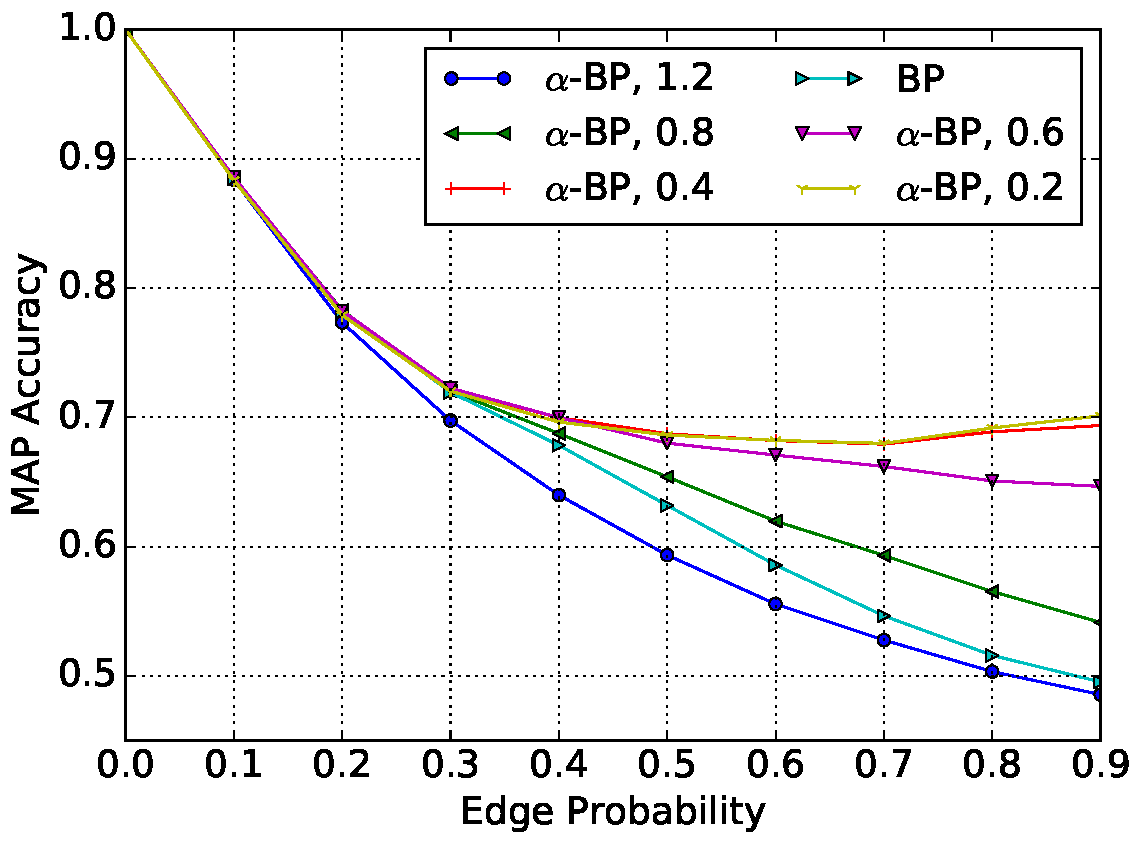
\includegraphics[width=1\linewidth]{figures/MAPacc_edgeP_sum_crop.pdf}
    \vspace{-0.6cm}
    \caption{Mismatch between MAP and $\alpha$-BP on\\ binary MRF}
    \label{fig:mismatch}
  \end{subfigure}
  \begin{subfigure}{.5\textwidth}
    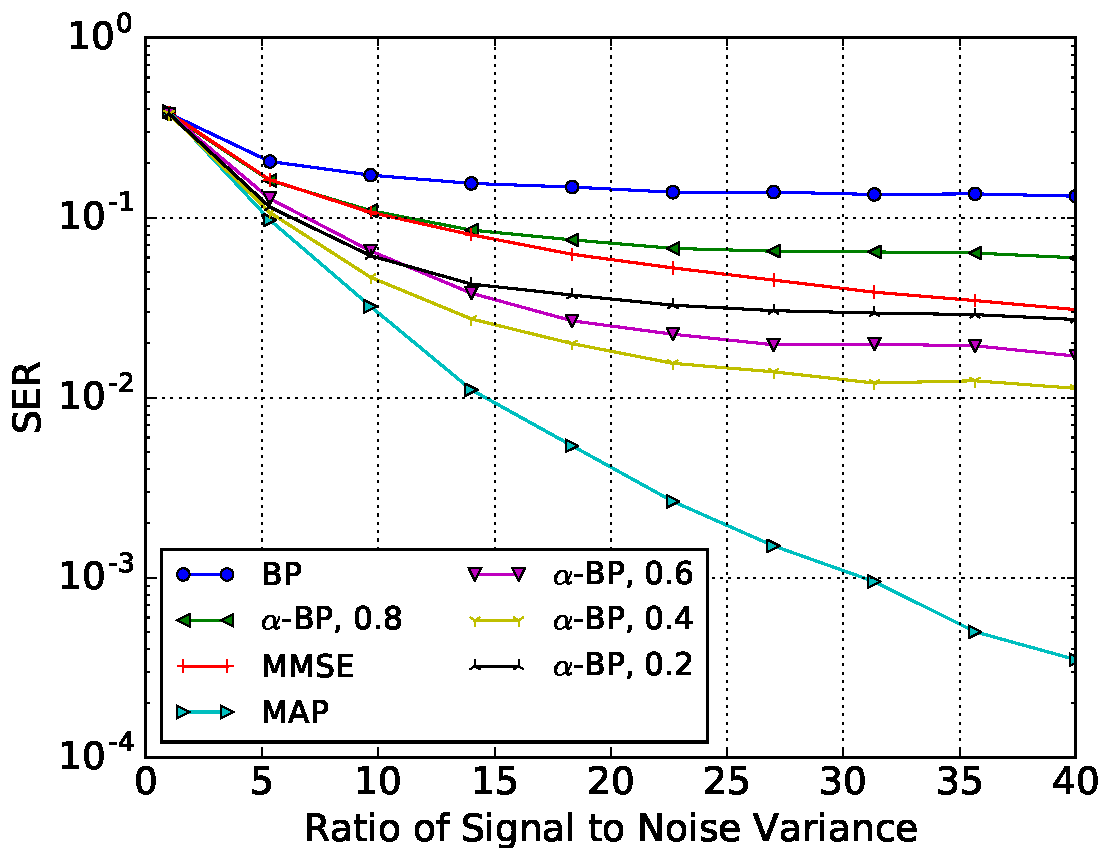
\includegraphics[width=1\linewidth]{figures/alpha_compare_crop.pdf}
    \vspace{-0.6cm}
    \caption{MIMO detection: $\alpha$-BP without prior\\~}\label{fig:mimo_a}
  \end{subfigure}
  \begin{subfigure}{.5\textwidth}
    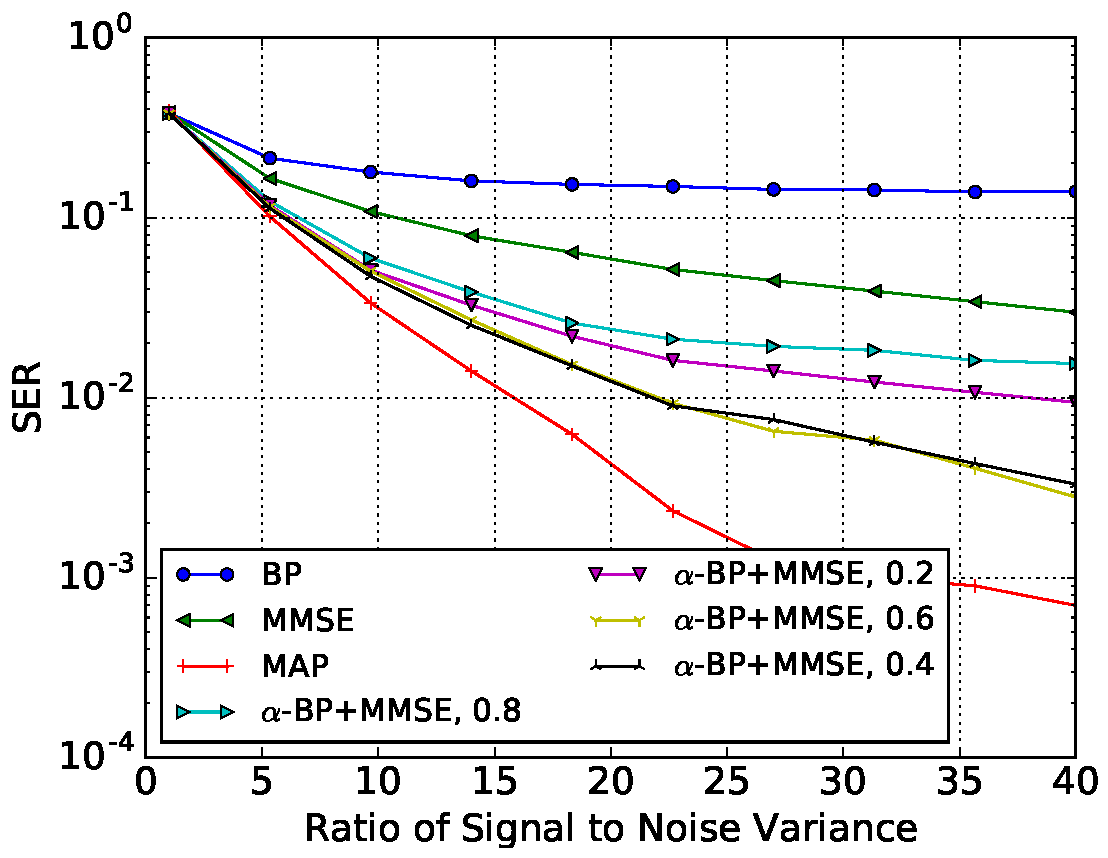
\includegraphics[width=1\linewidth]{figures/prior_mmse_alpha_compare_crop.pdf}
    \vspace{-0.6cm}
    \caption{MIMO detection: $\alpha$-BP with prior\\~}\label{fig:mimo_b}
  \end{subfigure}
  \vspace{-0.3cm}
  \caption{Numerical Results of $\alpha$-BP on: (a) binary MRF, (b) and (c) MIMO detection.}
  % \caption{MIMO detection in Comparison with MMSE and MAP: (a). $\alpha$-BP without prior; (b). $\alpha$-BP with prior from MMSE.}
  \vspace{0.3cm}
  \label{fig:mimo_detection}
\end{figure}

In this section, we report numerical results on the $\alpha$-BP. It is well known that performance of BP and its variants deteriorate significantly when loops appear in factor graph. We would like to see if $\alpha$-BP could relief the deterioration brought by loops in inference. Thus we firstly test the performance of $\alpha$-BP for MAP inference in a MRF with $\Aa=\{-1,1\}$ (Ising model), where we adjust how loopy its corresponding factor graph is.

In addition, we apply the $\alpha$-BP to a MIMO detection problem, to explore its performance in comparison with (loopy) BP and minimum mean square error (MMSE). At the end, the prior factor trick is used according to discussion in Subsection~\ref{subsec:remark}. This turns out to be MAP inference problem as well.

For the MAP inference, the most probable estimation by $\alpha$-BP, $\hat{\bm{x}}=[\hat{x}_1, \cdots, \hat{x}_N]$, is obtained by
\begin{align}
  \hat{x}_{i} = \uargmax{x_i}\tilde{f}_i(x_i) \prod_{k\in \text{Pa}[i]} m_{k\rightarrow i}(x_i), x_i \in \Aa.
\end{align}




With $t_k(x_i, x_j) = e^{-2J_{i,j}x_i x_j}$ and $f_i(x_i) = e^{-J_{i,i}-b_i x_i}$, \autoref{eq:mrf} can be reformulated as
\begin{equation}
  p(\bm{x}) \propto \exp\{-\bm{x}^{T}\bm{J}\bm{x} - \bm{b}^{T}\bm{x}\}, \bm{x} \in \Aa^N,
\end{equation}
where $\bm{x}^{T}$ is transform of $\bm{x}$, $J_{i,j}$ is element of symmetrix matrix $\bm{J}$ at $i$-th row and $j$-th column, $\bm{b} = [b_1, \cdots, b_N]^T$.


For this experiment, we set $\Aa = \left\{ -1, 1 \right\}$ and $N=9$. Bias $\bm{b}$ is sampled from Gaussian, ${b_i} \sim \Nn(0, (1/4)^2)$. Since $\bm{J}$ decides the loopy level of its corresponding factor graph, we use the Erdos-Rényi model \cite{erdos1960} to construct its connectivity. Namely, an element of $\bm{J}$ is set as non-zero, $ {J}_{i,j} = {J}_{j,i} \sim \Nn(0,1)$, with an \textit{Edge Probability}. Otherwise, ${J}_{i, j} = {J}_{j,i} = 0$, which means this is no connection between variable node $x_i$ and $x_j$. For each test value of Edge Probability, $5000$ binary MRF models are generated randomly and mismatch between $\argmax_{\bm{x}} p(\bm{x})$ and $\left\{ \bm{x}|\argmax_{x_i}q_i(x_i) \right\}$ is computed in each realization. The results are shown in \autoref{fig:mismatch}. As the Edge Probability increases, graphs become loopier and $\alpha$-BP (also BP) has more mismatch with MAP inference. In general, $\alpha$-BP with $\alpha > 1$ underperforms BP, and $\alpha$-BP with $\alpha < 1$ outperforms BP. For $\alpha=0.2, 0.4, 0.6$, $\alpha$-BP stops deteriorating for Edge Probability increasing over $0.35$, while BP continues giving even worse approximations.

\begin{figure}[!t]
  \begin{subfigure}{1\textwidth}
    \captionsetup[subfigure]{justification=centering}
    \centering
    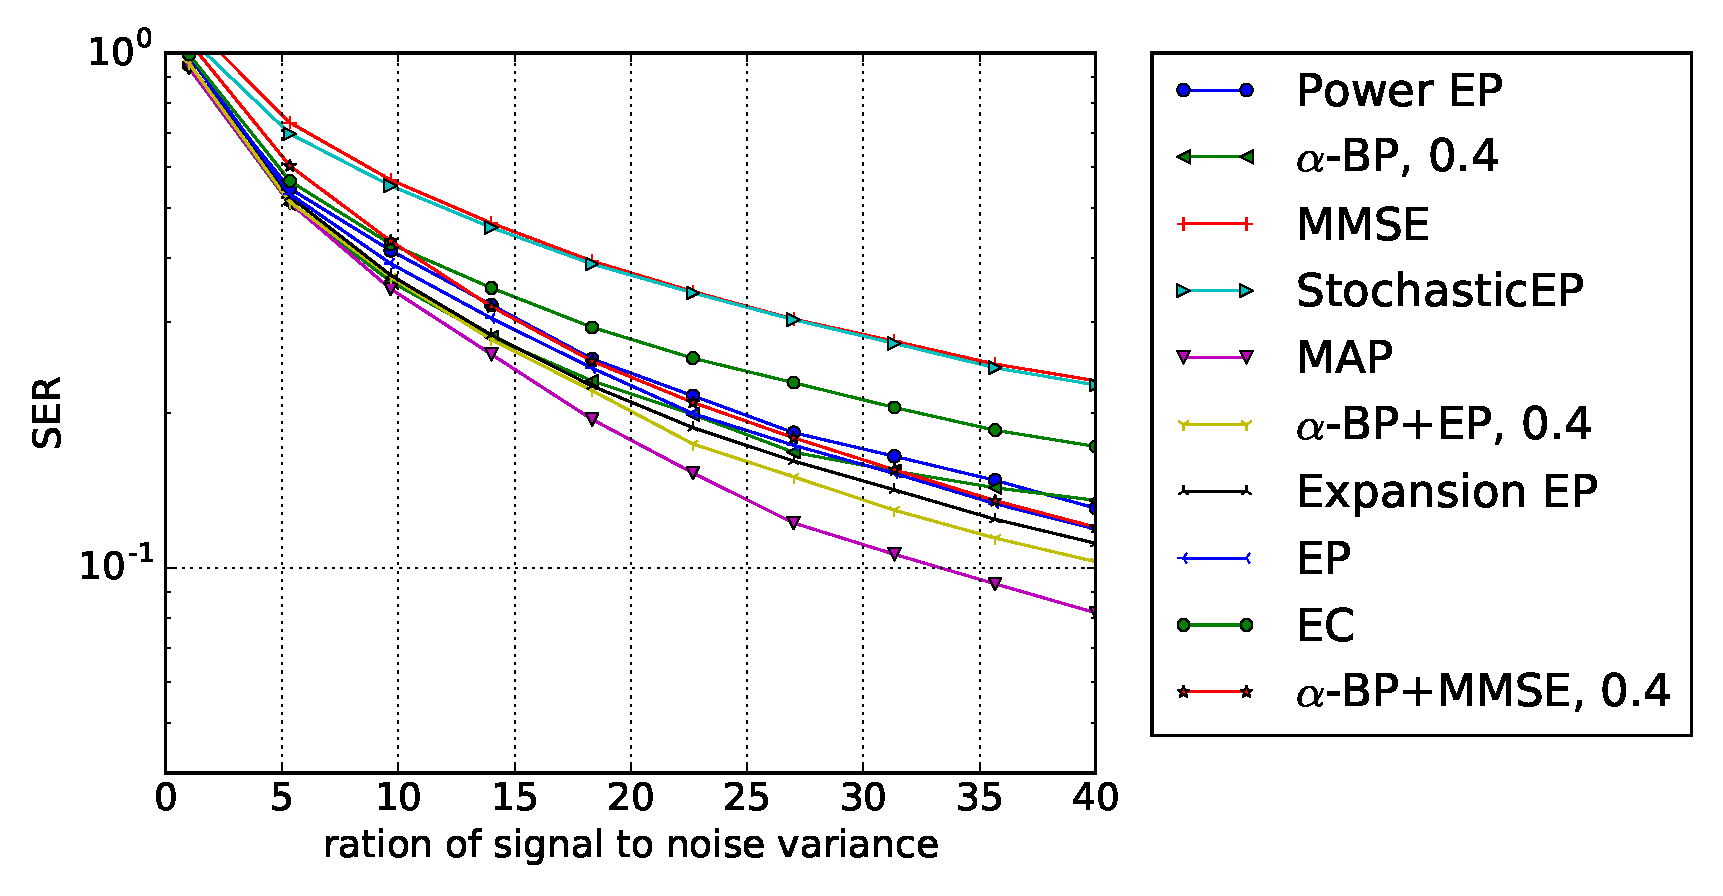
\includegraphics[width=1\linewidth]{figures/ep_experiments4by4_qpsk_alpha4_.eps}
    \caption{Scenario: input size 4, ouput size 4.}
    \label{fig:compare-const4-44}
  \end{subfigure}
  \begin{subfigure}{1\textwidth}
    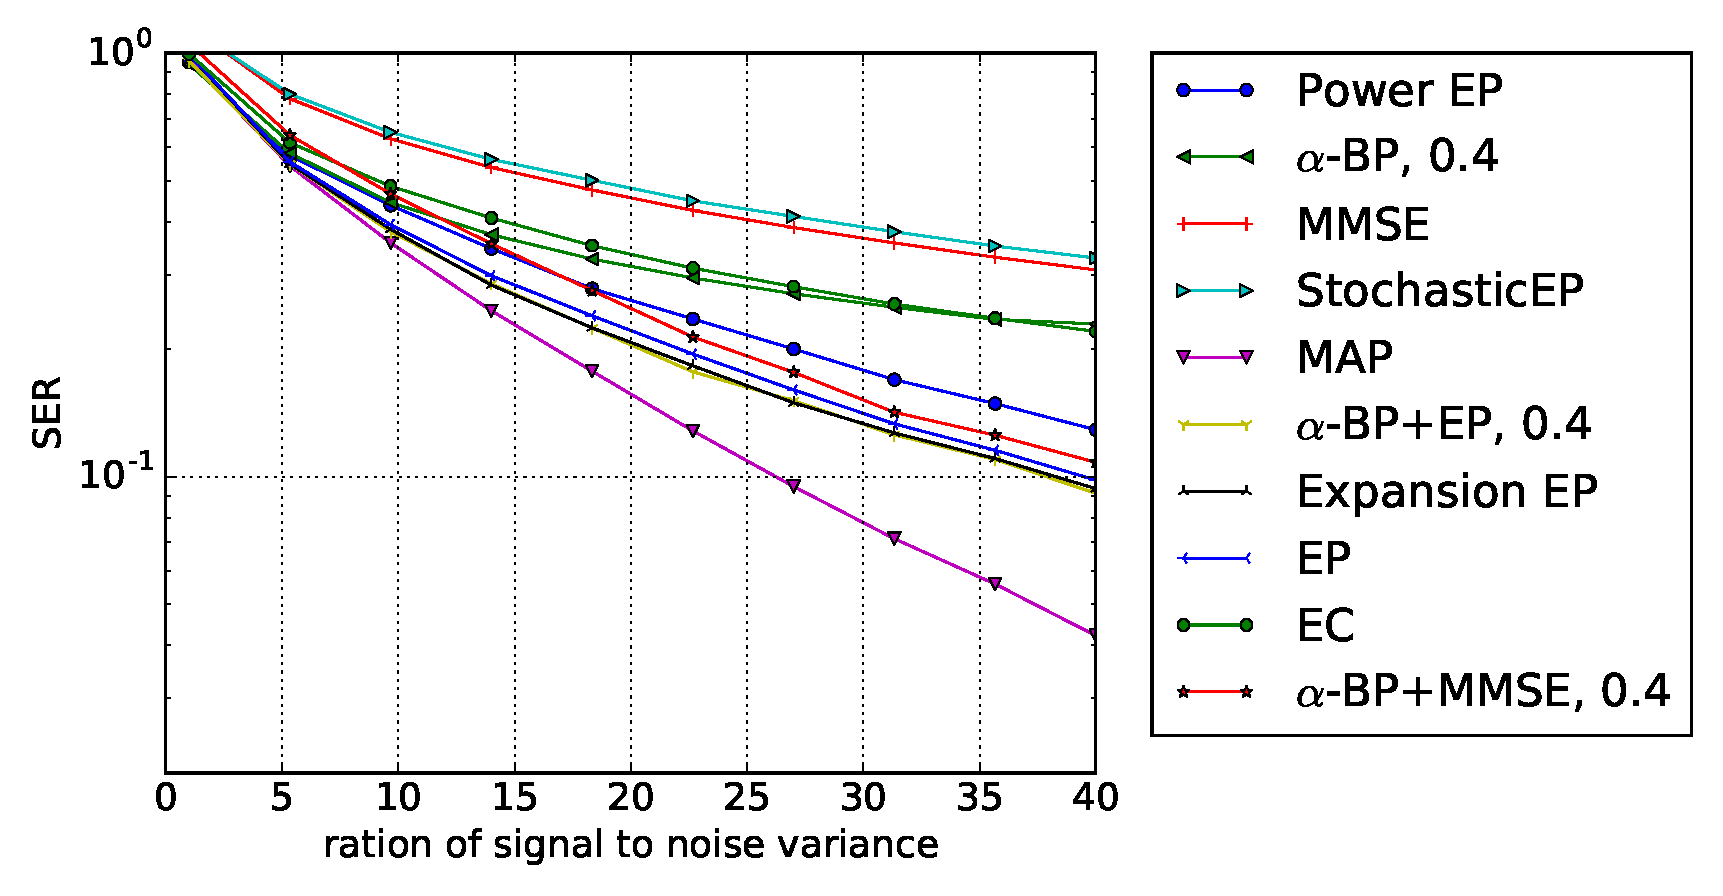
\includegraphics[width=1\linewidth]{figures/ep_experiments8by8_qpsk_alpha4_.eps}
    \caption{Scenario: input size 8, ouput size 8.}
    \label{fig:compare-const4-88}
  \end{subfigure}
  \caption{Numerical results of discussed algorithms, constellation
    size 4.}
  \label{fig:compare-const4}
\end{figure}
\begin{figure}[!t]
  \begin{subfigure}{1\textwidth}
    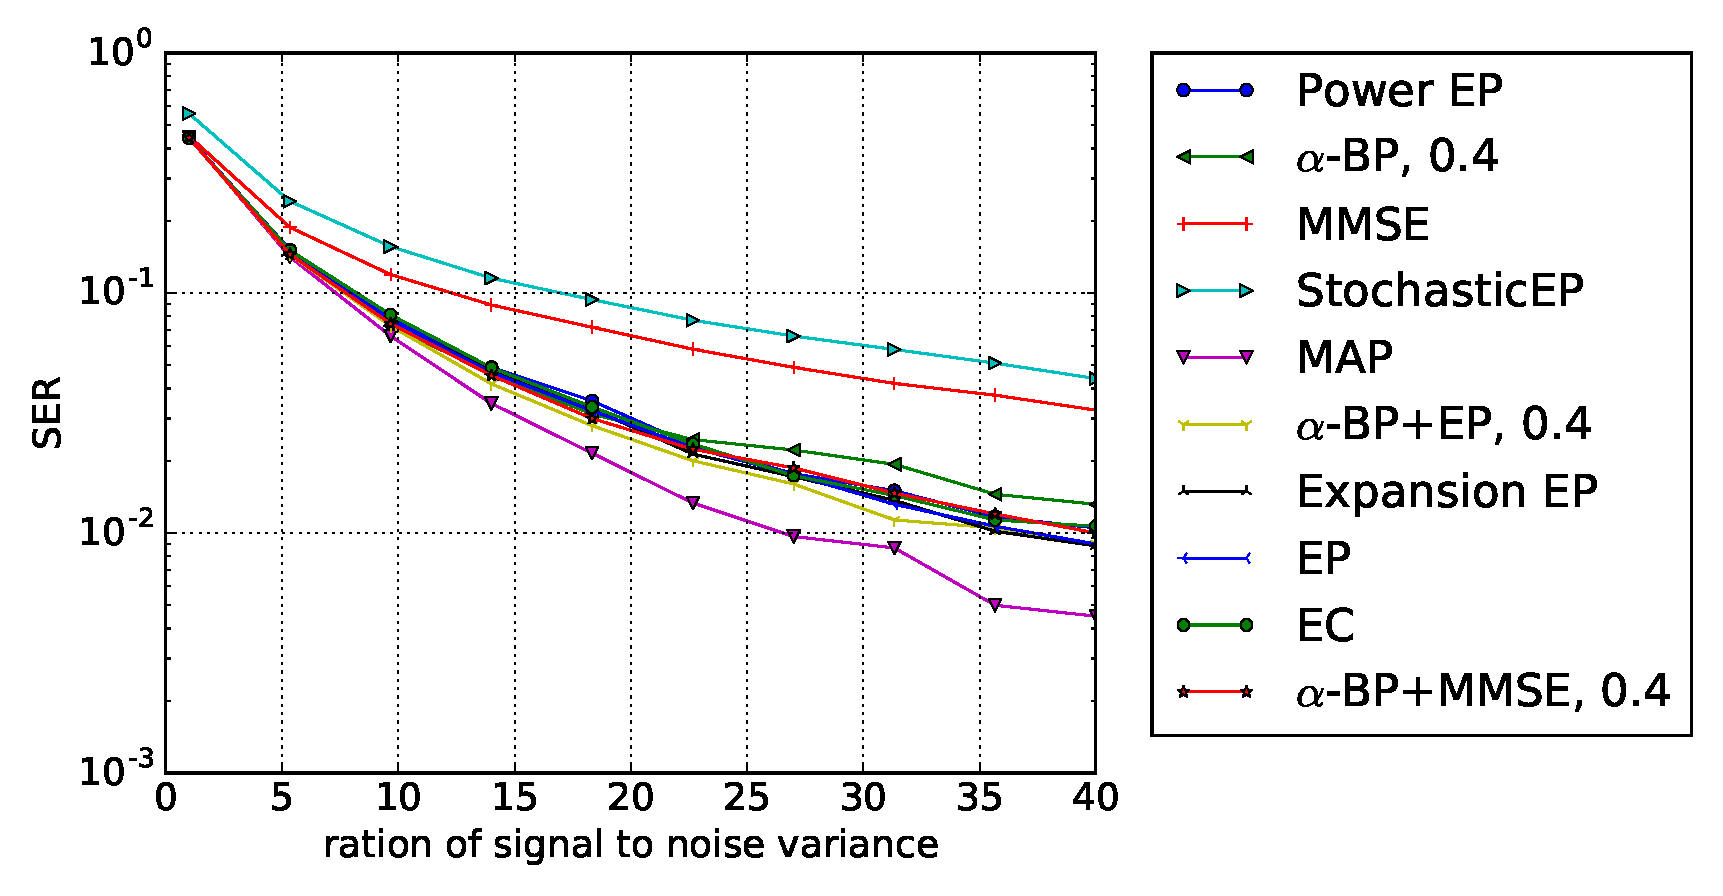
\includegraphics[width=1\linewidth]{figures/ep_experiments_4by4_bpsk_alpha4.eps}
    \caption{Scenario: input size 4, ouput size 4.}
    \label{fig:compare-const2-44}
  \end{subfigure}
  \begin{subfigure}{1\textwidth}
    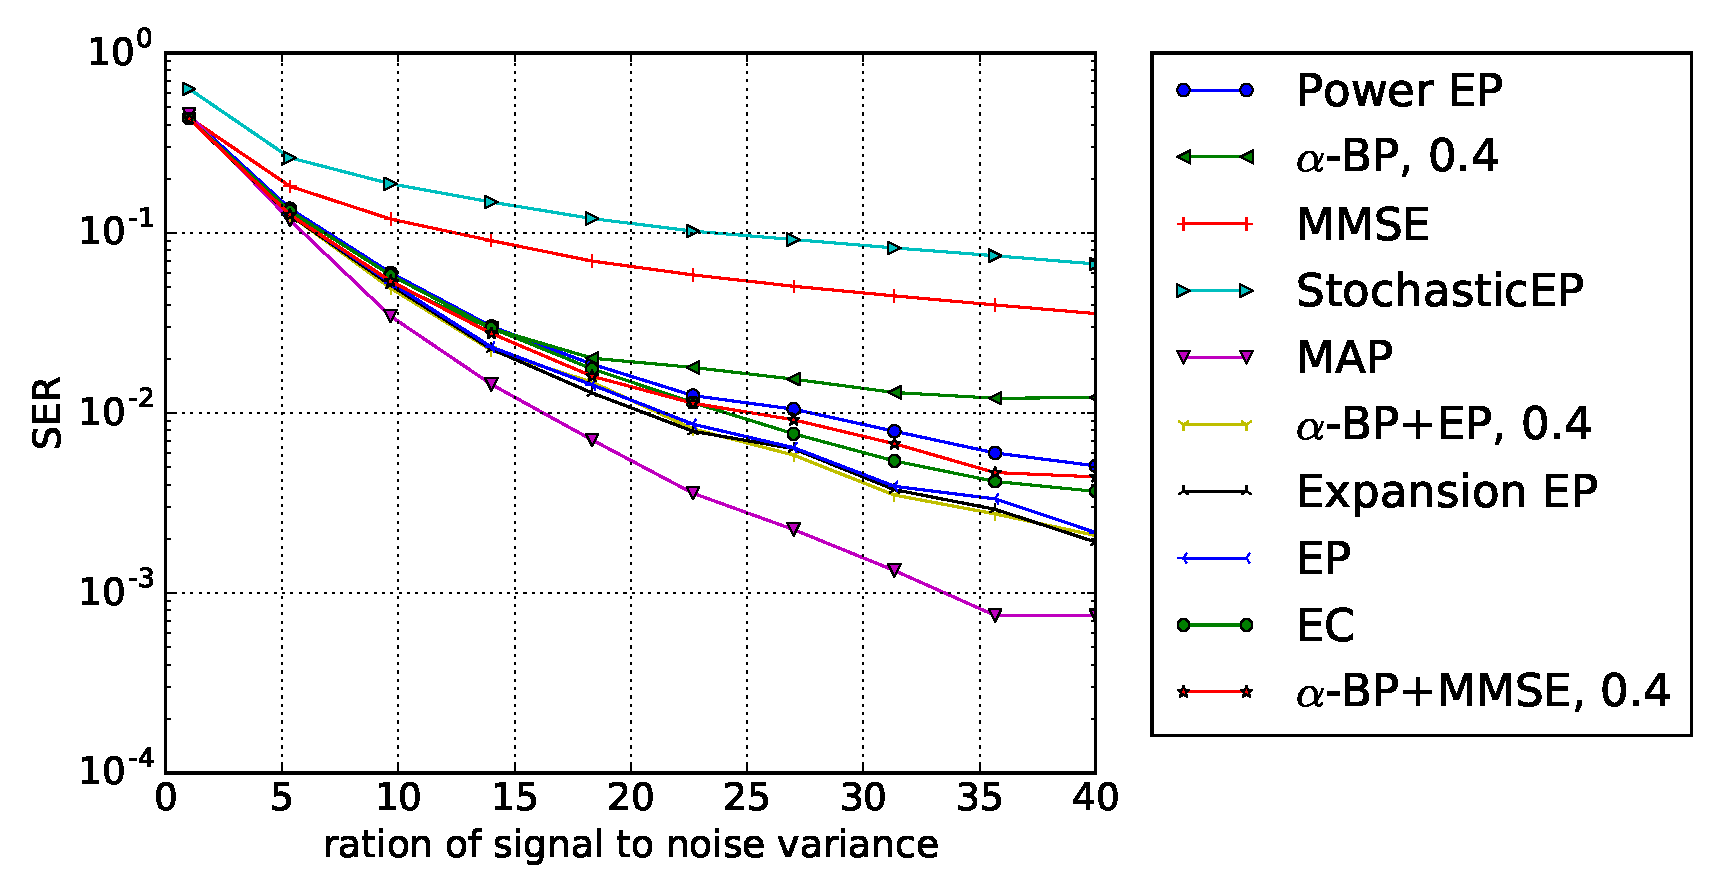
\includegraphics[width=1\linewidth]{figures/ep_experiments8by8_bpsk_alpha4.eps}
    \caption{Scenario: input size 4, ouput size 4.}
    \label{fig:compare-const2-88}
  \end{subfigure}
  \caption{Numerical results of discussed algorithms, constellation size 2.}
  \label{fig:compare-const2}
\end{figure}
\section{Numerical Results}


In this section, we made a comparison between the algorithms discussed in this report. The software written for this set of experiments is implemented in Python. The algorithms implemented includes MMSE, expectation propagation, stochastic expectation propagation, power expectation propagation, expansion expectation propagation (correction of expectation propagation), and some improvement tricks. The maximum a posterior is used shown numerically as a reference bound for all algorithms.

The legends explanation for corresponding algorithm are shown as in Table~\ref{tab:lagend}.
\begin{table}[h]
  \caption{Legend Explanation}\label{tab:lagend}
  \centering
  \begin{tabular}{ |p{3cm}||p{8cm}|  }
    \hline
    MMSE   & Minimum Mean Square Error \\
    \hline
    EP   & Expectation Propagation (Section~\ref{sec:EP}) \\
    \hline
    Power EP & Power Expectation Propagation (Section~\ref{sec:power-ep}) \\
    \hline
    Expansion EP & Expansion Expectation Propagation (The First-order Expansion in Section~\ref{sec:imporveEP}) \\
    Stochastic EP & Stochastic Expectation Propagation (Section~\ref{sec:stochasticEP}) \\
    \hline
    EC & Expectation Consistency (Section~\ref{sec:ec}) \\
    \hline
    $\alpha$-BP & $\alpha$ Belief Propagation (Section~\ref{sec:alphabp}) \\
    \hline
    $\alpha$-BP$+$MMSE & $\alpha$-BP assembled with MMSE as prior (Section~\ref{subsec:assemble,subsec:remark}) \\
  \end{tabular}
\end{table}

\bibliography{myref}
\bibliographystyle{plain}

\end{document}


%%% Local Variables:
%%% mode: latex
%%% TeX-master: t
%%% End:
